\chapter{The Language of Spices}
\label{ch:language}


% Discussion Chapter
% Discuss and relate your findings to the literature review and theory framework.
% Do so in such a way that a layperson can understand your argument.
% How do the findings relate to the theory and methods discussed previously?
% Why you have reached particular conclusions?
% How do your findings relate to the gaps in the literature you identified earlier?
% What implications do the findings have for the discipline and for existing understanding?
% How do the findings relate to your research questions, aims and objectives?

%------------------------

% This chapter presents an inquiry with classic corpus linguistic methods into spicy words

% This chapter presents the various ways spice terms have established themselves in our daily language, illustrating that they --- some more than other --- are deeply embedded in the collective human experience. From the earliest of times, since humans started to uses spices as medicine, incense, perfume, and condiments, they left their mark in our vocabulary. This, of course, includes fluctuations varying by region and historical periods, and certain substances enjoyed a higher esteem than others at any given time. 

% My hypothesis is that the more a... 



% \section{Spices in Corpora}

% distribution/frequency

% different spices are more prevalent in different languages/cultures, showing their importance

% mention hindi?

% spoken corpora?

% \subsection{}

% word sketches

% modifiers modified
% what can we learn

% \subsection{Historical Corpora}

% some diachronic comparison?

% \section{Spice Terms and Word Classes}

% use sketch engine to check for adjectives then verbs

% \subsection{Spice Terms as Adjectives}

% spicy

% peppery

% salty?

% \subsubsection{Spices Names as Colors}



% \subsection{Spice Terms in the Verb Paradigm}

% to spice up

% to pepper

% \section{Spices as Metaphors and in Idioms}

% doukou is virgin/maiden age

% 虎辣人 hularen peppery or short-tempered person 395 defrancis

% then check metaphors and idioms

% to have pepper in the nose
% hungarian paprikas hangulat

% different spices in different cultures

% Examples:

% https://en.wiktionary.org/wiki/%E8%B1%86%E8%94%BB


% %------------------------------------------
% \section{\textsc{Spice} in language}

% \subsection{English}

% \subsection{Chinese}

% 辣 s.v. ① peppery; hot ② sharp; spicy; biting (of smell/taste) ③ vicious; ruthless 
% defrancis 525



\section{The Case of Pepper}

One of the most globally and cross-linguistically recognizable words of the spice domain is \textit{pepper}. In the \gls{WOLD}, it is ranked no. \nth{7} when sorted by borrowability, following behind the olive, the sugar, the wine, the kettle, the beer, and the cheese, in the semantic field of food and drink \autocite{wold}. Pepper has a score of 0.66, making it the top spice meaning in this dataset of 81 entries (and the only spice besides the chili pepper). This metric, ``borrowed score'', is an average of the scores of all the words that correspond to the meaning `pepper', where individual meanings are scored according to their borrowed status.\footnote{The values assigned are determined as the following: clearly borrowed: 1.00, probably borrowed: 0.75, perhaps borrowed: 0.50, very little evidence for borrowing: 0.25, and no evidence for borrowing: 0.00. See more at \url{https://wold.clld.org/terms}} ``Thus, the higher the average borrowed score of a meaning, the greater its borrowability.'' -- it is explained on the database's website. This suggests that if we were to collect the words for pepper in different languages and project them onto a world map, we should be able to see clusters that indicate the donor languages, and that gather around key areas of the globe that were important in the diffusion of this spice and \gls{wanderwort}. This in turn, would highlight the cultures and locations that were responsible for its transfer.

\subsection{The Distribution of Pepper}

Similarly to the analysis we conducted in \cref{ch:diffusion} with cinnamon and the distribution of its names seen in \cref{fig:cinnamon_distribution}, we can also plot the names of pepper onto a world map, and look at how they are dispersed at present. First, I made the choice to collect words that correspond to `pepper', and not compounds that gloss the more specific `black pepper' (or not `chili pepper' for that matter). Then, I have collected the names by scraping the relevant Wiktionary translations\footcite{noauthor_pepper_2022} for the word \textit{pepper} in the sense `spice', (and not in the sense of `fruit of the capsicum'). I then cleaned and manually checked the data for errors, and corrected the list to the best of my ability. Next, I augmented the dataset using other sources, such as dictionary entries, \textcite{katzer_spice_2012}, and the ``the pepper'' meaning page from \gls{WOLD} by \textcite{wold}, which contains 36 entries. Lastly, I have analyzed the words based on their etymologies, and grouped them into categories according to their etymons. After concatenating the collected data with language information and coordinates obtained from the \gls{WALS} and \gls{Glottolog} datasets, the plot could be generated, and it can be found under \cref{fig:distribution_pepper}

\begin{figure}[!ht]
    \centering
    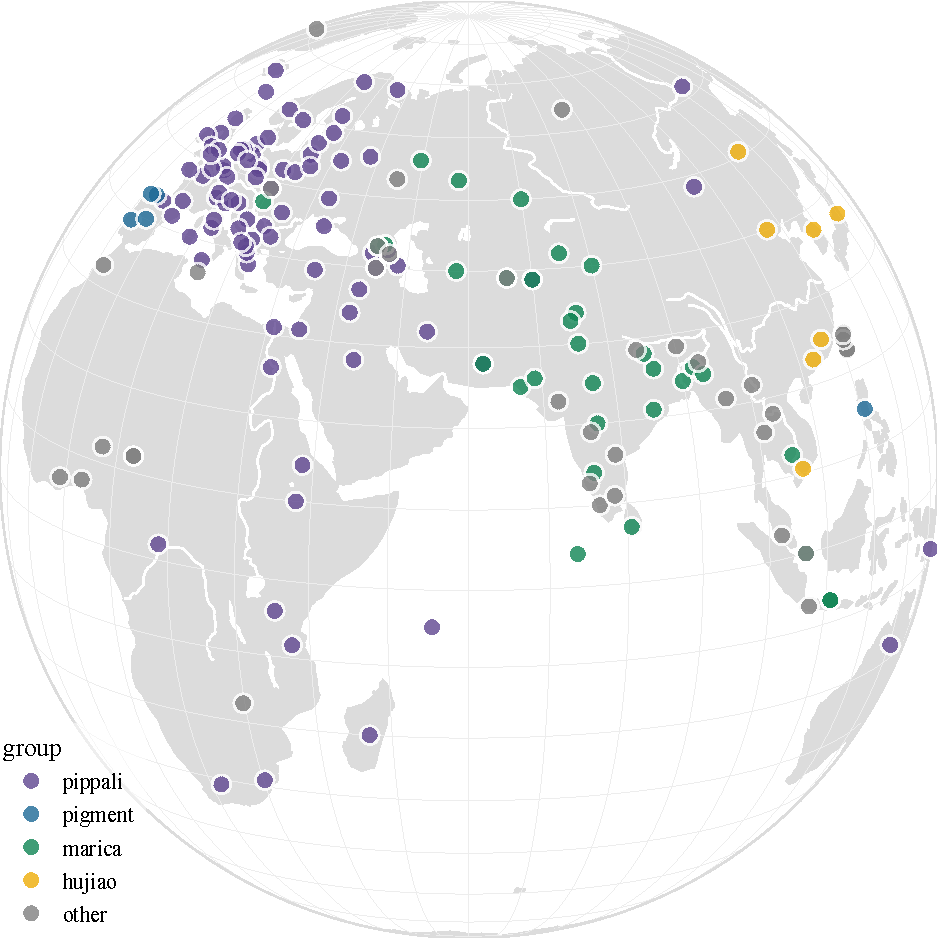
\includegraphics[width=\linewidth]{imgs/plots/distribution_pepper.pdf}
    \caption[The distribution of names for pepper (\taxon{Piper nigrum}).]{The distribution of names for pepper (\taxon{Piper nigrum}) in a few languages around the globe. For a full, interactive and explorable version of the plot, please visit the following link: \url{http://htmlpreview.github.io/?https://github.com/partigabor/phd-test/blob/main/distribution_pepper.html}.}
    \label{fig:distribution_pepper}
\end{figure}

Looking at \cref{fig:distribution_pepper} it becomes immediately evident, that there are a few large, clearly distinguishable groups forming among the scattered data points, each representing a word and a language. The following categories were identified: pippali, pigment, marica, and hujiao. Pippali contains all words that ultimately derive from Sanskrit \textit{pippali} and this means most languages in Europe, including those that were influenced by Latin \textit{piper}, and those that loaned this word through Persian \textit{pilpil} and Arabic \textit{fulful}. The pigment group covers West Iberian Romance languages, where the Latin word for pigment went through a series of changes by way of metonymy and specialization of meaning, explained under \ref{ety:pimento}. The marica groups captures instances that originate in the ``true sense'' for black pepper, Sanskrit \textit{marica}, which is distributed across South, Central, and to a lesser extent Southeast Asia. Lastly, words that belong to the hujiao group are those languages that borrowed their word for black pepper from Chinese, found across the Sinosphere. 
% every group that has at least
% three attested members???
% What's the threshold?
Instances that do not belong to any group or their origins I could not determine were assorted to ``other''. Besides the apparent category of words derived from Sanskrit \textit{pippali} (and spread generously though Persian and Latin), there are other major and minor groups that can be discerned, especially the category of words that derive from Sanskrit \textit{marica}. The piquancy of this ambivalence in the distribution of these two Sanskrit words is elevated by the fact that while \textit{pippali} refers to long pepper (\taxon{Piper longum}), \textit{marica} is the term that originally referred to black pepper (\taxon{Piper nigrum}) --- forming a duo of closely related aromatic plants and spice terms.

Words that derive from \textit{marica} are dispersed throughout South and Central Asia, and Hungarian \textit{bors} is probably the furthest instance geographically from the once Sanskrit heartland and the home of pepper. Hungarian tribes most likely loaned this word from Turkic speaking peoples (with many other words from the domain of commerce and agriculture) on their way to the Carpathian basin sometime before the \nth{9} century.\footnote{Hungarian \textit{bors} was attested in 1075 as a proper noun, 1395 as a common noun. Cf. Ottoman Turkish dialectal \textit{burç}, Chuvash \textit{pərəs} `id.', the Turkic words are from an Iranian language; cf. Sogdian \textit{marč}, Pamirian \textit{märč} `id.' \autocite[90]{zaicz_etimologiai_2006}}



We know for a fact that even in the early times of the Roman republic (510-31 \BC{}), Indian long pepper was imported and used in Europe, but have evidently lost its prominence later on. From the history of this word, we can ascertain that at the time the Greeks borrowed the word for pepper from Aryan merchants, long pepper was definitely traded alongside black pepper. Unfortunately, we are not sure in what ratio they were imported, but they were both knows to ancient writers of Europe. Hippocrates have discussed pepper and its medicinal benefits in the \nth{5} century \BC{}, Theophrastus have distinguished them in his \textit{Historia Plantarum} in the \nth{4} century \BC{}, and explained the difference between the two; stating that long pepper has a stronger flavor. According to \textcite{toussaint-samat_history_2009}, the pepper that the Romans preferred was in fact long pepper, and the round black peppers we now use ``became popular in the \nth{12} century and had replaced long pepper by the \nth{14}''. It is often difficult to know which pepper ancient writers are talking about, because in Latin, both could be referred to simply as \textit{piper} \autocite[442-443]{toussaint-samat_history_2009}. The modern scientific names go back to these early times, \textit{longum} means `long' and \textit{nigrum} means `black'. 

If we rely on historians, it becomes rather trivial that the name \textit{piper} and its other derivatives is a \gls{wanderwort} that have first traveled with the product (the long pepper called \textit{pippali}), and went through a semantic shift later, when black pepper replaced long pepper. The word stayed, but its referent changed. And this change happened alike in many languages in this part of the world, even if the the two kinds of peppers looked different, their flavor profile and functions were the same. This semantic change happened once more in history: when people became acquainted with chilies, the same shift happened, and people started to use their (local) words for the pepper they had, to refer to the red hot chili peppers that conquered the world.

% More on this on the pepper conundrum. 
%section here?

% The situation is also interesting in Thai, where the word for pepper was \tha{พริก} \textit{phrík} `pepper', a Khmer donation from Sanskrit \textit{marica} present for the 12-\nth{14} centuries. However, this term refers to chilies today. The arrival, success, and integration of the New World chilies into Thai culture and cuisine forced people to make a distinction between the old and new peppers, and so the Asian black pepper became known \tha{พริกไทย} \textit{phríkthay} [pepper-Thai], meaning `Thai pepper' \autocite{suthiwan_thai_2009}.

%...
% discuss marica in data

%explain situation about pepper fulful jiao cabai, and chilies

% \section{The Pepper Conundrum: Act I}


\subsection{The Diffusion of Pepper}

The names of pepper on the above map demonstrate indirect evidence for the trails the material have left, and show the extent of trade networks at certain times. They reveal the cultures and civilizations located at the heartland of the product and the crossroads of its exchange. The distribution of clusters of words belonging to the same categories in this plot also indicate the possible ways of diffusion. This can be then studied from a historical linguistic point of view through investigating language contact and loanwords, reinforced with historical awareness, and supported by botanical information. Domain knowledge of spices is also crucial, if we want to answer specific questions about the spread of spices and spice terminology. For example, one of the reasons pepper (and its name) was so successful on reaching faraway places so early on is due to the fact that pepper does not spoil. Or at least, not fast compared to other agricultural products; it keeps it aroma and pungency longer that many other spices. \textcite[59]{krondl_taste_2007} writes that ``pepper, in particular, is remarkably stable and can be stored up to a decade as long as it’s kept reasonably dry.'' This is one of the key feature of spices, that allowed them to be shipped and carried thousands of miles away, during the course of several months if not years. Moreover, as dried plant matter, spices are also light, resulting in an extremely high price-to-weight ratio compared to, say, wheat, which made trading in pepper so lucrative in the past, and defined the fate (and face) of cities, such as Venice.

Turning our attention back to vocabulary, the most fascinating part of this phenomenon is that the word \textit{pepper} originates so distant from English; both in time and space. Thanks to the hard work of historical linguists and philologists, we have a decent reconstruction of \textit{pepper}'s journey, and we know that Germanic tribes must have loaned the term on mainland Europe, some time before their migration to England around the \nth{5} century. early Old English \textit{pipor} comes from Latin, which originates in the Sanskrit word \textit{pippali} by way of an Indo-Aryan transmission (see \ref{ety:pepper}). The spatial and temporal trajectories of this word are remarkable, and follow the path of the material. Indian pepper (black and long) was known and coveted in Arabia and Rome long before the Anglo-Saxons got to taste it. Still, much of the story of pepper and its worldwide diffusion goes back to prehistoric times. Tracing its itinerary on Eurasian pathways is difficult at this time depth, yet we have breadcrumbs: its names. \textit{Pippali} and its derivatives mark the way the spice have spread, even where written documentation and archaeological finds are missing.

\begin{figure}[!ht]
    \centering
    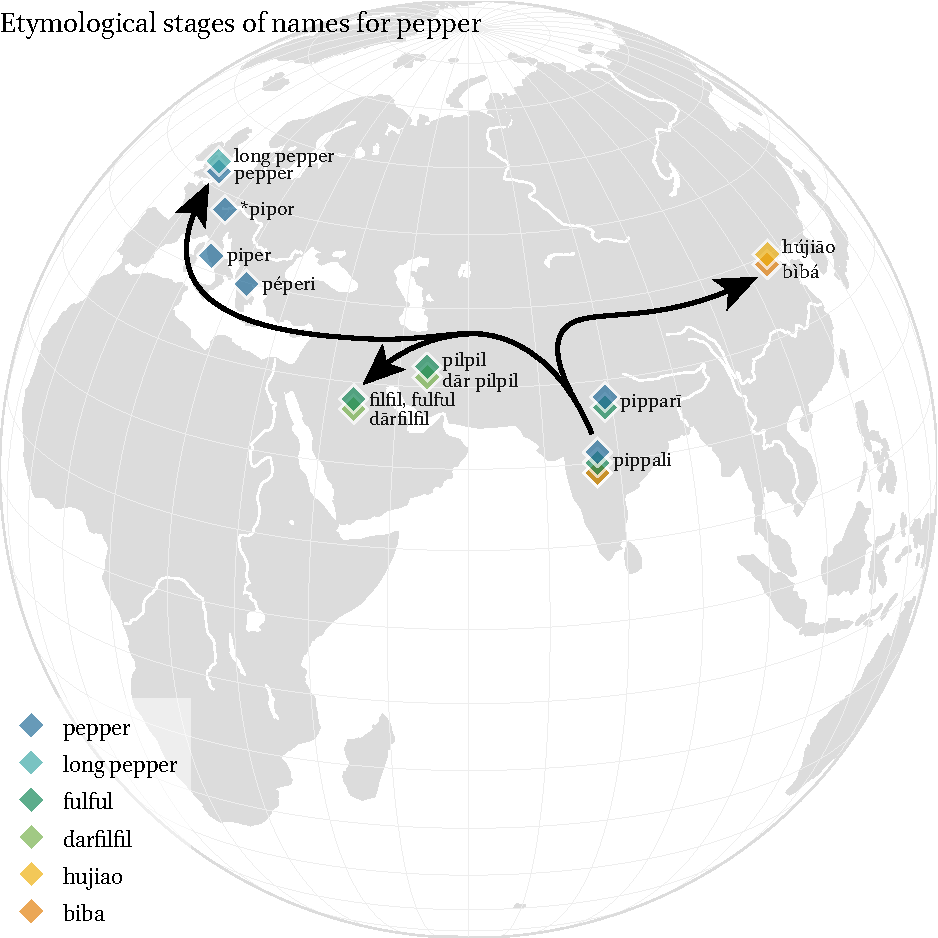
\includegraphics[width=\linewidth]{imgs/plots/diffusion_pepper_edited.pdf}
    \caption[The diffusion of names for pepper.]{The diffusion of names for pepper (\taxon{Piper nigrum; P. longum}) in English, Arabic, and Chinese. For a full, interactive and explorable version of the plot, please visit the following link: \url{http://htmlpreview.github.io/?https://github.com/partigabor/phd-test/blob/main/diffusion_pepper.html}.}
    \label{fig:diffusion_pepper}
\end{figure}

Now, homing in on our scope of English, Arabic, and Chinese, we can look at the etymological stages of the words for pepper in these languages. In \cref{fig:diffusion_pepper}, I tried to illustrate the origins of the words for pepper in the languages under inspection. We see that the branch that leads to English is on the same trajectory as Arabic, both going back to the Sanskrit etymon. They also formed their words for long pepper with the prototype words \textit{pepper} \& \textit{filfil}: English modeled it after Latin, while Arabic loaned a Persian term that compounded `wood' and `pepper' (\textit{dar pilpil}), the reasons behind which we can only speculate. Either it reminded the Persians to a piece of stick, or there was maybe some type of analogy with the name of cinnamon: \textit{dar chini}. Unmistakably, the Chinese did not loan a word for black pepper pepper, they formed their own name by compounding their prototype word, \textit{jiao}, appending it with \textit{hu}, referring to foreigners, Western barbarians. Notwithstanding, Sanskrit \textit{pippali} also survives in Chinese, in the form of \textit{biba}, strictly referring to long pepper, known since ?? and still used in \gls{TCM}. The questions begs to be asked: Why was one pepper adopted with a native word and designation, and why was the other loaned? I can think of two reasons. First, black peppercorns are very similar to the indigenous Sichuan peppers --- in their shape, size, taste, and function --- therefore it seems obvious to apply the term that already exist and conceptually very close to the new material. By way of their similarity, a metaphoric way of expression extended the set of referents for this word, \textit{jiao}. Second, long pepper was a new item not incredibly similar to already existing Chinese products, it would place itself further away from Sichuan pepper in the semantic space. They do not match in color, shape, size, and even in its use long pepper was (and still is) rather a medicine than culinary spice. It was alien enough to be adorned with a loanword.

% “Foreign pepper”. The principal time of import to China was estimated to be during the Tang dynasty, and the source―per the miscellany Miscellaneous Morsels from Youyang of the 9th century CE―was the Magadha Kingdom of India, where it was called 昧履支 (MC muʌiH liɪX t͡ɕiᴇ) locally; cf. Sanskrit मरिच (marica, “black pepper”).

The etymologies were introduced in detail under etymologies \ref{ety:pepper}, \ref{ety:fulful}, and \ref{ety:hujiao}.

% Put attestation dates on maps!!!
% That would be cool

\subsection{The Role of Pepper in English: A Brief Contemplation About Spiciness}

Now that we have discovered that pepper as a product, and thus \textsc{spice} as a concept was at one point a novelty for the ancestors of English speakers, let us briefly consider life before pepper. We can safely presuppose a time, where pepper --- and therefore experiences of spiciness --- simply did not exist for certain communities. Or did it? Was there some wild garlic growing in Europe whose sharpness in taste could be compared to pepper? Some mustard, or horseradish? How did these people describe spiciness before spice? Or peppery before pepper? 

Sensory experiences of taste, such as sweet, salty, sour, and bitter, are encoded in the mappings of our evolutionary biology, and the same is true for pain. In fact, spiciness is a tactile sensory experience, roughly working along the same mechanisms as our perception of heat and pain. The technical term is chemesthesis, and it is defined as the sensitivity of our mucosal surfaces of the skin (e.g. the moist inner linings of the mouth) to outside chemicals. This system activates thermal, nociceptive (i.e. pain), and tactile sensations \autocite{simons_oral_2008}. Substances such as piperine (in black pepper) and capsaicin (in chile pepper) cause a reaction that activates this system causing a burning, stinging sensation which --- in moderate amounts --- can be a pleasant. These stimuli also contribute to the overall flavor perception of food \autocite{tewksbury_evolutionary_2008}. The first sense of the word \textit{pungent} (now rare) shows well how strong the connection to pain was: ``of pain: as if caused by a sharp point; piercing, stabbing; pricking.'' The definition for the sense that is now generally understood is ``affecting the sense organs, esp. those of smell or taste, with a sharp, penetrating sensation; acrid, irritant; intensely flavored, piquant.'' Words, such as \textit{pungent}, \textit{sharp}, \textit{biting} (also a cognate of \textit{bitter}), and \textit{hot} show that we do not necessarily need the word \textit{spicy} (a loanword), to describe \textsc{spiciness} (i.e. pungency). However, the foreign concept of \textsc{spice} was influential enough to make way for new words and meanings attested in \nth{13} century English. 

%spice, spicy...

Today, spices and their access ability is taken for granted, and the idea of not knowing how ``spicy'' tastes like, is --- for most of us --- unimaginable. The existence and abundance of spices around us, even if one does not prefer the heat on a daily basis, is now part of the human experience. This omnipresence is reflected in our words; spices have become the part of our vocabulary, the way we speak, and not just when we talk about the spices themselves. The following section will show how spices infiltrated our language, and how their characteristic features gave rise to new words and new meanings, metaphors, and idioms. I will examine the profound effect spices made on the lexis, through looking at the case of pepper in English.

\section{\textit{Pepper} as a Lexical Item}

Pepper, and I mean black pepper, is undoubtedly a prototypical spice. In a significant portion of the world's regions --- or at least in the temperate areas --- black pepper was the first pungent spice people have ever tasted. Although black pepper became indeed the first global spice, it is not the only one. Many other regions have their own prototypical pungent spices and relishes; some already famous worldwide, some still relatively unknown. As examples, we must mention the chile of the Americas, the prickly ash of China, the \textit{cabai} of Southeast Asia, and the grains of paradise of West Africa. Now, if I would to list them again in the same order, but this time through a finer/different sieve of English, I could have written: chili pepper, Sichuan pepper, long pepper, and melegueta pepper. Mind you, these are all botanically different aromatic plants, distributed all over the globe, all culturally rooted in their respective regions. Yet in English, all of them can be referred to as some kind of pepper. 

What we have here, is evidence that English speakers, going beyond the primary sense of the term \textit{pepper} (used for the little round fruits of \taxon{Piper nigrum}) have developed the use of this word for ``any of certain other pungent spices derived from plants of other families, esp. ones used as seasonings''\footcite[pepper, n.]{oed}. The meaning of \textit{pepper} was extended by ways of its physical attributes (small, black, seed-like fruits), chemical characteristics (pungency), and role (spice, seasoning, condiment). Hence, other substances that matched or approximated one or more of the above-mentioned features, could be referred to as \textit{pepper}. Often with a distinguishing word, today many plant products are known as peppers: \textit{red}, \textit{pink},  \textit{bell}, \textit{sweet},
\textit{Jamaica}, \textit{alligator}, etc. The list is long and functionally diverse, as distinguishing words and modifiers can have various different roles. They can identify, distinguish, or indicate some aspect of the produce, for example, its place of origin, flavor, or shape. \textit{Pepper}, with the primary meaning referring to the fruits of \taxon{Piper nigrum}, was attested in early Old English, and the extended sense developed shortly after the European ``Age of Exploration'', when the world opened up to the English sailors and merchants, and exotic, new products were brought back from Africa, Asia, and America. A \nth{16}-century quote from a herbal shows this new use of the word \textit{pepper}, and also the attitude towards a novel spice --- Guinea pepper\footnote{An ambiguous name for an African source of ``pepper'', it can refer to one of three different spice yielding plants: \taxon{Aframomum melegueta} (grains of paradise, melegueta pepper, etc.); \taxon{Piper guineense} (West African pepper, Ashanti pepper, etc.); \taxon{Xylopia aethiopica} (Grains of Selim, Senegal pepper, etc.)} --- and simultaneously hints on the status of black pepper: 

\begin{quote}
``Ginnie pepper hath the taste of pepper, but not the power or vertue.'' \\
(Gerard, J. (1597) \textit{Herball} (Vol. 2, p. 293).in \cite[pepper]{oed})
\end{quote}

And so, a \textit{pepper-genesis} started, a rather clumsy term I made up for this phenomenon when Europeans familiarized themselves with new additions from the fruits of the plant kingdom; both to the cargo hold of their ocean-going ships, their apothecaries and grocers, and their vocabularies. Pepper worked as a prototype, and lent its name to other fragrant plant materials that needed to be named, 

% Analyze pepper names here

Beyond this the ability to generate names of all kinds of peppers --- true and false --- there is an even more interesting aspect of the word \textit{pepper} that I would like to discuss: the derivation of new words over various word classes.

% grammatical categories

\cdot

We also assume that the more a language is familiar with a substance, more senses could exist in a language, and with this above assumption (4) we look for derivationally related linguistic categories of terms from the spice domain. Under these categories we will include:

the names (nouns)
• names of the sensation induced by the spice (nouns, adjectives)
• synaesthetic properties associated with the spice (adjectives, verbs)
• cognate verbs of seasoning, cooking (verbs)
• denominal metaphors, idiomatic expressions (nouns, verbs, phrases)

\begin{figure}[ht!]
    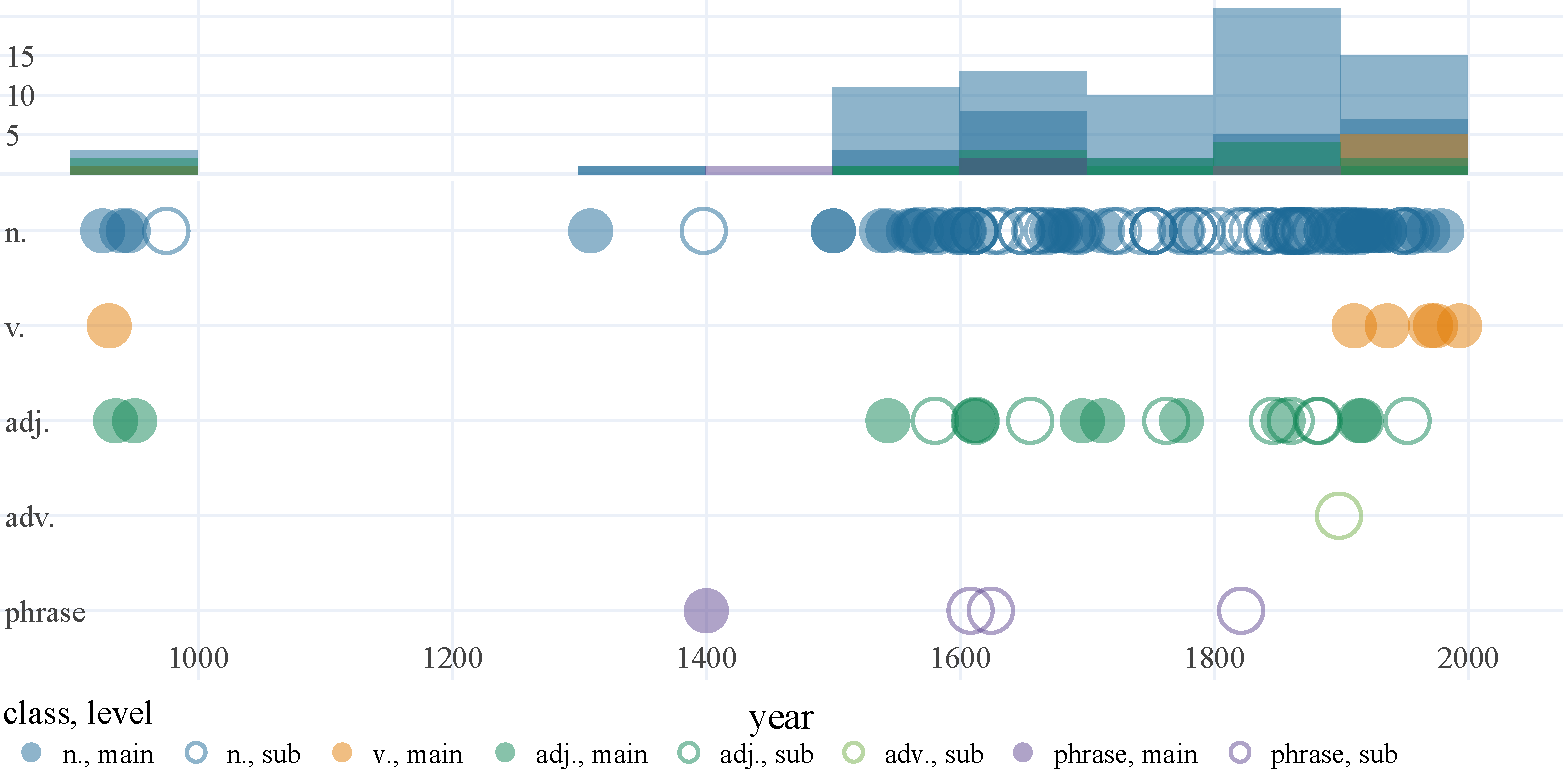
\includegraphics[width=\linewidth]{imgs/plots/oed_pepper.pdf}
    \caption[A timeline of words and phrases derived from pepper.]{A timeline of words and phrases derived from \textit{pepper}, based on main- and sub-level entries in the OED, and plotted by the dates of their attestations. A histogram on the top margin shows the number of attestations in 50 year increments. To explore the data points in an interactive plot, please visit the following link \url{http://htmlpreview.github.io/?https://github.com/partigabor/phd-test/blob/main/oed_pepper.html}.}
    \label{fig:oed_pepper}
\end{figure}








The English compound ‘pep talk’ appeared in colloquial American English in the 20th century, and contains ‘pep’, which is a shortening for pepper, meaning “energy and high spirits; liveliness, vigour, power” (OED). We can see the WordNet mappings showing ‘ginger’ as one of the synonyms for ‘pep’, and consulting a dictionary confirms the evidence of a second spice representing ‘liveliness’: “Spirit, pep, energy; temper. Frequently in to put ginger (into), to show ginger.” (OED), in American slang.


We suspect that word frequencies in corpora would show their relative importance in a language, hence for example ‘Sichuan pepper’ and its variations34 in an English corpus should have a smaller relative frequency (0.03 per million words), than ‘花椒’ huājiāo (“Sichuan pepper”) in a Chinese corpus (4.6 per million), or ‘हल्दी’ haldī (“turmeric”) in a Hindi corpus should have a very high frequency score (27.29 per million words), which arguably shows the importance of this spice in Indian culture. These are merely examples from the preparatory stage, but similar observations shall be refined and collected in a tasteful and readable manner in the dissertation.